
\documentclass{article}

\PassOptionsToPackage{numbers,sort&compress}{natbib}
\usepackage[preprint]{模板/neurips_2026}

\usepackage{fontspec}
\usepackage[UTF8]{ctex}
\setmainfont{TeX Gyre Termes}

\usepackage{hyperref}
\usepackage[T1]{fontenc}
\usepackage[utf8]{inputenc}
\usepackage{amsmath,amssymb}
\usepackage{graphicx}
\usepackage{booktabs}
\usepackage{array}
\usepackage{multirow}
\usepackage{caption}
\usepackage{longtable}
\usepackage{enumitem}
\usepackage{xcolor}
\usepackage{adjustbox}
\usepackage{float}
\usepackage{placeins}
\usepackage{xurl}

\hypersetup{
  colorlinks=true,
  linkcolor=black,
  citecolor=blue!50!black,
  urlcolor=blue!50!black
}

\captionsetup{font=small,labelfont=bf}
\setlist[itemize]{leftmargin=1.2em}
\setlist[enumerate]{leftmargin=1.5em}
\setlength{\emergencystretch}{2em}
\raggedbottom

% Figure placeholder for paper drafting.
\newcommand{\figureplaceholder}[2]{
  \fbox{
    \begin{minipage}[c][#2][c]{0.95\linewidth}
      \centering
      \textbf{图位预留}\\[0.5em]
      \footnotesize #1
    \end{minipage}
  }
}

\title{DermAgent: A Structured Agentic Reasoning Framework on Top of Frozen Dermatology Vision-Language Backbones}

\author{Anonymous Authors}

\begin{document}
\maketitle

\begin{abstract}
本文聚焦的不是“如何再训练一个更强的皮肤科视觉语言模型”，而是一个更具体的问题：在固定骨干模型的条件下，能否通过结构化的 test-time 智能体推理提升最终诊断质量。皮肤科多模态诊断不仅依赖视觉识别，还依赖比较、排除、病程演化判断、风险评估、不确定性审计以及对既往经验的调用。现有视觉语言模型虽然能够直接给出结论，但其诊断过程大多以内隐生成方式完成，临床关键推理动作难以显式审计，跨病例经验也难以沉淀为可复用、可冻结评测的外围能力。本文提出 DermAgent，一种面向皮肤科诊断的结构化智能体推理框架。DermAgent 的定位不是替代骨干视觉语言模型，而是在保持骨干模型作为唯一最终诊断者的前提下，于最终诊断前增加一层结构化、可审计的 test-time 推理支架。

DermAgent 将整体系统组织为一个完整的诊断智能体，而不是一个孤立的“证据增强模块”：骨干模型先完成初始视觉感知，智能体中间层再执行经验检索、技能选择、技能执行、证据组织与状态更新，最终仍由骨干模型基于结构化证据包生成诊断结论。在这一框架中，技能被定义为原子化临床推理动作而非病种分类器；经验被划分为原始病例记忆、战术经验与抽象经验；认知状态与策略层则分别承担跨病例偏好统计与当前病例控制决策。由此，系统能够在冻结骨干模型的条件下，对技能选择、经验检索、证据组织与控制策略进行独立优化，同时保留经验积累与策略演化的结构基础。与直接对骨干模型进行大规模微调相比，这种优化重点转向外围策略层的路线在资源需求上更克制，也更容易将形成的经验与策略状态以可复用资产的形式保留下来。

在同骨干、同病例列表与冻结评测条件下，DermAgent 在 345 个测试病例上将直接 Qwen 基线的 top-1 准确率从 29.6\% 提升至 39.7\%，将恶性召回率从 48.2\% 提升至 82.2\%，并将错误率从 70.4\% 降至 60.3\%。配对统计进一步表明，top-1 提升具有统计显著性（McNemar 精确检验，$p=0.0035$），恶性召回提升极为显著（$p=3.68\times10^{-22}$）。阶段性实验显示，基础临床推理技能已能贡献主要增益，而分层经验、认知更新与控制器驱动的技能压缩进一步改善了稳定性、风险识别与推理效率。结果表明，在固定皮肤科视觉语言模型骨干的前提下，结构化智能体推理是一条有实证支持的增强路径，但其收益主要体现为更好的最终判断质量与高风险纠错，而非对所有指标的无条件同步提升。
\end{abstract}

\section{Introduction}

皮肤科诊断并非单纯的图像分类问题，而是一个高度依赖视觉表型、临床上下文与鉴别诊断逻辑的多步决策过程。即使单张病灶图像已经提供了较强的视觉线索，临床判断通常仍需围绕病灶形态、颜色模式、边界与表面特征、病程演化、患者背景信息以及恶性风险信号进行逐步收缩式推理。对于黑色素细胞病变、角化性病变及若干高混淆病种而言，局部外观相似、metadata 不完整、时间信息缺失以及风险信号与表面视觉线索不一致等因素，都会显著增加诊断难度。因而，皮肤科智能诊断不仅要求模型“看懂图像”，还要求其能够显式处理病程演化、风险与信息缺口，并以可审计的方式组织临床推理。

近年来，通用视觉语言模型以及面向医学场景的多模态大模型为皮肤科智能诊断带来了新的可能性。这类模型能够在统一接口下处理图像、文本与部分临床元数据，并生成观察描述、鉴别候选及解释性文本，因此相较于传统专病分类器，更接近开放式临床推理的交互范式\citep{skingpt4_2024,panderm_2025,skingptr1_2025,skinr1_2025,skinflow_2026}。然而，对于本文所关心的固定骨干增强设定，这类模型在实际诊断中仍面临三个关键限制：其一，推理过程通常以内隐生成方式完成，难以确认模型是否显式执行了比较、排除、不确定性评估、病程演化判断与信息缺口检测等关键临床动作；其二，在高混淆、高风险或信息不足病例上，单次生成往往难以稳定地区分“证据尚不足”与“结论已经足够成立”；其三，直接提示很难形成跨病例复用的经验结构，也难以把历史错误、混淆模式与策略偏好沉淀为可训练、可审计的外围能力。概括而言，当前真正的痛点不是模型不能生成答案，而是模型缺少一个在 test-time 显式组织临床推理与沉淀经验的中间层。

一种自然的改进方向是通过提示或提示链对基础模型施加额外约束，例如要求模型先描述病灶，再给出鉴别诊断，最后输出结论。尽管此类方法实现简洁，也常能带来一定收益，但其控制粒度通常仍停留在输出格式或浅层步骤提示上，难以把“哪些推理动作应被触发”“哪些历史经验应被检索”“哪些证据应进入最终诊断上下文”显式建模为独立对象。更重要的是，这类方法往往缺少可跨病例累积的长期状态：一次推理中产生的有效技能、典型混淆对或高价值经验片段，很难在后续病例中以结构化形式复用。因此，这类系统仍更接近一次性问答，而不是能够在 test-time 逐病例组织证据、并在长期尺度上累积经验的临床推理框架\citep{xskill_2026,tarse_2026,autoagent_2026}。从系统实现角度看，这也意味着其改进路径往往要么继续堆叠 prompt engineering，要么回到对骨干模型本体进行更重的训练，而较难在冻结骨干条件下形成资源更节制、经验可复用的外围增强路线。

这促使我们进一步考虑结构化智能体推理的必要性。对于皮肤科诊断，更合理的方向不是让外围模块直接输出病种标签，而是把若干具有清晰临床语义边界的局部推理动作外显化，并围绕最终诊断前的证据构建发挥作用。沿着这一思路，技能可以被定义为原子化临床推理动作，例如形态分析、颜色模式分析、边界与表面审查、病程演化判断、鉴别比较、排除推理、恶性风险评估、不确定性评估以及信息缺口检测；经验不应仅是相似病例缓存，而应进一步区分具体病例记忆、战术层经验和跨病例抽象经验；在此基础上，还需要一种跨病例的认知状态，用于记录混淆模式、技能帮助性、检索偏好和策略倾向，使技能选择、经验选择与证据组织从静态模板转变为可演化的外围策略层\citep{xskill_2026,tarse_2026,macro_2026,memskill_2026,autoagent_2026}。本文并不把这些元素作为并列堆砌的模块来宣称贡献，而是明确把它们都收束到同一条主线上：为最终诊断前的 structured evidence 构建服务。

然而，在引入智能体推理时，另一个同样重要的问题是系统边界。如果将外围模块设计成多个子诊断器，再通过投票或聚合决定最终病种，系统很容易退化为多模块投票式诊断框架；如果将技能写成若干刚性的启发式分类器，则又会把结构化推理简化为外挂式规则分类器。基于这一考虑，本文刻意避免三类路线：多模块投票式诊断、刚性启发式分类器外挂，以及非冻结、非同条件的智能体与基线对比。更具体地说，DermAgent 被定义为一个完整的诊断智能体，但这个智能体在职责上受到严格约束：它负责组织证据、选择动作、检索经验与维护状态，却不直接给出最终疾病标签；最终诊断责任始终明确保留给底层视觉语言模型本身。

基于上述观察，本文提出 DermAgent，一个面向皮肤科诊断的结构化智能体推理框架。DermAgent 的核心思想是：由智能体承担经验驱动的技能组织、经验检索、证据路由、状态更新与 test-time 推理计算。由此，本文关注的核心问题可以明确表述为：\textbf{在固定皮肤科视觉语言模型骨干的条件下，结构化、经验驱动的智能体推理是否能够优于直接提示？} 该问题的重点不是“能否再训练出一个更强的皮肤科模型”，而是“在保持同一骨干不变时，结构化智能体中间层本身是否具有独立增益”。进一步地，本文还明确把 skill 与 experience 的跨病例积累视为方法卖点的一部分：我们关心的不只是一次推理里能否组织证据，也关心有效动作与有价值案例能否被沉淀为可复用的 skill/experience 资产，而不是每次都从零开始组织推理。

本文的主要贡献如下：
\begin{enumerate}[leftmargin=1.8em]
  \item 提出 DermAgent，一种面向皮肤科诊断的结构化智能体推理框架，在固定骨干视觉语言模型的前提下，将最终诊断前的临床推理显式组织为技能、经验、认知与证据四个相互配合的层次。
  \item 将技能建模为原子化临床推理动作，将经验建模为原始病例记忆、战术经验与抽象经验的分层体系，并显式区分经验内容、认知状态与策略控制层，从而支持可审计的证据构建，以及 skill/experience 在跨病例尺度上的积累与复用。
  \item 设计了严格的冻结评测协议，在同骨干、同病例列表与关闭在线写回的条件下，公平比较直接基线与不同智能体变体，并利用阶段性实验、组件消融、配对统计与定性案例分析系统验证方法有效性。
  \item 在固定 345 个测试病例上的受控实验表明，DermAgent 能显著提升 top-1 准确率与恶性召回率，并在专用皮肤病大模型 SkinVL 上保持可迁移的增益，说明围绕冻结骨干构建资源更节制、经验可复用的结构化智能体推理层，是增强皮肤科视觉语言模型的有效方向。
\end{enumerate}

\section{Related Work}

\subsection{皮肤科视觉语言模型与推理模型}

近年来，面向皮肤科场景的视觉语言模型与领域专用多模态模型逐渐成为医学 AI 的重要方向。SkinGPT-4、PanDerm、SkinGPT-R1、Skin-R1 与 SkinFlow 等工作分别从通用多模态交互、foundation model、reasoning-oriented tuning 与流程化推理等角度推动了皮肤科大模型的发展\citep{skingpt4_2024,panderm_2025,skingptr1_2025,skinr1_2025,skinflow_2026}。这些研究共同表明，皮肤科 AI 的核心挑战已不再局限于闭集分类，而越来越转向开放临床情境中的视觉--语言推理质量、风险识别能力以及诊断过程的可信性。

\subsection{医学智能体与工具增强推理}

随着大模型智能体框架的发展，医学场景中也出现了越来越多围绕工具调用、流程分解与多步推理展开的方法。这类工作通常通过检索器、知识库、规则工具、外部计算模块或多轮规划机制，使模型在单次回答之外具备更强的任务分解与证据整合能力\citep{healthcare_agents_review_2026}。不过，现有医学智能体很多仍然集中在文本问答、文献检索、报告生成或通用医疗咨询等任务上。DermAgent 的定位并非纯文本医疗问答助手，而是一个专门服务于皮肤图像诊断的结构化推理层；并且在系统责任分工上，它始终保持骨干模型作为唯一最终诊断者，而不把智能体变成新的最终决策者。

\subsection{基于技能与经验的智能体学习}

XSKILL 与 TARSE 提供了与 DermAgent 最直接相关的方法学启发。它们共同强调，skill 与 experience 应被显式区分：skill 更像可复用的动作能力或过程模板，experience 则更像与历史实例相关的轨迹、条件和反馈信号\citep{xskill_2026,tarse_2026}。与此同时，MACRO 与 MemSkill 进一步推动了这一方向的发展，分别强调从历史成功执行中发现可复用程序，以及把 memory operation 本身重写为可选择、可演化的 skills\citep{macro_2026,memskill_2026}。

\subsection{认知演化、记忆与自我改进智能体}

AutoAgent、MemSkill 等工作强调，agent 若要在长程任务中持续提高适应性，就不能只依赖静态 prompt，而需要维护跨回合的结构化 cognition、压缩与抽象 memory，以及基于结果反馈的闭环更新\citep{autoagent_2026,memskill_2026}。DermAgent 借鉴了这一思想，但在医学诊断场景中更强调 frozen evaluation、state isolation 与在线 writeback 的严格边界。

\subsection{DermAgent 的方法定位}

综上，DermAgent 位于皮肤科视觉语言模型、医学智能体、技能/经验学习与认知演化的交叉点。与重新训练新骨干模型或构造通用医疗问答智能体不同，本文关注的是：在固定皮肤科视觉语言模型骨干的条件下，如何通过结构化的外围推理层提升最终诊断质量，并保持过程可审计、可分解和可公平评测。

\section{Method}

\subsection{问题定义}

本文研究皮肤科多模态诊断中的结构化推理增强问题。给定一张皮肤病灶图像以及可选的临床 metadata，例如年龄、部位、病灶直径、症状变化与部分病史信息，系统需要输出最终诊断及相关解释信息。与直接将输入一次性送入视觉语言模型并要求其给出结论的设定不同，本文关注的问题是：在底层视觉语言模型保持不变的前提下，能否通过一个结构化、经验驱动的 agent 中间层，为最终诊断前的推理过程提供可审计、可训练且可公平比较的 structured evidence 增强。

形式上，可将系统记为
\begin{equation}
y = F_{\mathrm{backbone}}(x, m, \mathcal{E}(x,m;\theta_{\mathrm{agent}})),
\end{equation}
其中 $x$ 表示皮肤图像，$m$ 表示可选 metadata，$F_{\mathrm{backbone}}$ 表示固定的视觉语言模型，$\mathcal{E}$ 表示由 agent 产生的 structured evidence package，$\theta_{\mathrm{agent}}$ 则对应 planner、retrieval scoring、evidence calibration 等外围策略参数。

\subsection{整体方法概述}

DermAgent 的核心思想不是在骨干模型外再叠加一个并行诊断器，而是把整个系统组织为一个受边界约束的诊断智能体：骨干模型先完成初始视觉感知，智能体中间层再围绕当前病例执行经验检索、skill 选择、skill 执行、证据组织与状态更新，最终仍由骨干模型基于整理后的 evidence package 输出诊断。换言之，DermAgent 是一个完整 agent，而“证据增强”只是该 agent 在最终诊断前执行的关键步骤之一，而不是它的全部。

之所以采用这一流程，而不是让骨干模型直接一步生成最终答案，原因在于皮肤科诊断中的关键临床动作并不天然等价于一次性文本输出。病灶观察、病程演化判断、鉴别比较、排除推理、风险评估、不确定性审计以及对既往混淆模式的参考，本质上对应若干不同的局部 reasoning operations。若将这些动作全部留在一次性生成内部，它们既难以审计，也难以在冻结骨干的条件下独立优化。相反，将其外显为技能、经验、认知与证据组织过程，可以把原本内隐的诊断中间层转化为可检查、可训练、可冻结比较的外围推理支架。也就是说，本文采用这一流程并不是因为“多步流程看起来更复杂”，而是因为皮肤科诊断中确实存在若干需要分别建模的中间临床动作，而这些动作共同决定最终诊断前的证据质量。

因此，DermAgent 的整体流程可概括为“初始感知—结构化证据构建—最终诊断”三阶段：骨干视觉语言模型首先对输入图像及 metadata 进行初始视觉理解，生成病灶概述、初始鉴别候选与不确定性线索；随后，agent 基于该初始感知结果执行经验检索、skill 选择、skill 执行与证据组织；最后，骨干模型在读取整理后的 evidence package 后输出最终诊断。该流程的设计目标不是替代 backbone，而是在最终诊断前构建一层结构化、经验驱动且可审计的推理 scaffold。

% ================= Figure suggestion =================
% 图1建议放“整体框架图”：
% 内容应包括：输入病例 -> backbone初始感知 -> skill/experience/cognition驱动的
% planner/controller -> evidence package -> backbone最终诊断。
% 这张图的作用是让读者在进入方法细节前先建立全局心智模型。
\begin{figure*}[t]
  \centering
  \IfFileExists{figures/image5.png}
    {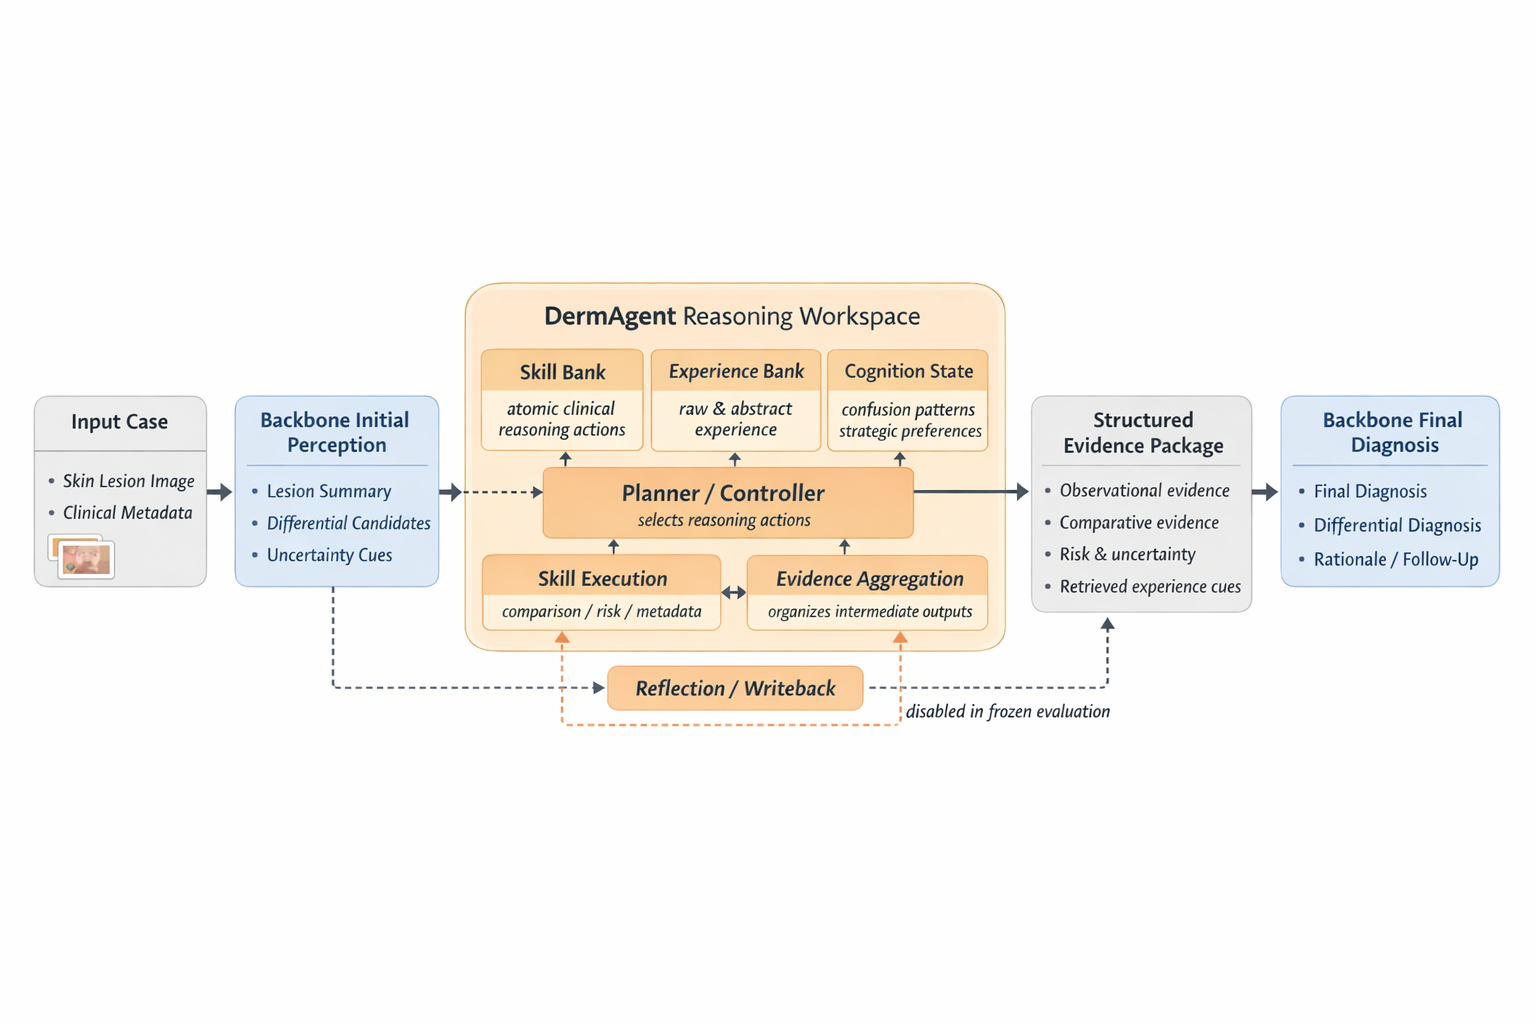
\includegraphics[width=0.9\textwidth]{figures/image5.png}}
    {\figureplaceholder{图1文件缺失：figures/image5.png}{0.24\textheight}}
  \caption{DermAgent 的整体框架。系统首先由骨干模型完成初始视觉理解，随后通过技能库、经验库与认知状态驱动的规划器/控制器选择并执行临床推理动作，最终将多源结构化证据组织为结构化证据包并送入骨干模型完成最终诊断。图中的虚线路径表示仅在训练或非冻结模式下启用的反思/写回闭环，在冻结评测中该路径被关闭。}
  \label{fig:overall}
\end{figure*}

\subsection{设计原则}

DermAgent 的方法设计遵循五项原则：单一最终诊断者原则、structured evidence 原则、经验与认知分层原则、外围可训练而骨干冻结原则，以及公平评测原则。系统始终保持骨干模型作为唯一最终诊断者；agent 既不直接输出最终疾病标签，也不通过投票或 override 取代 backbone 决策，而只负责构造对最终诊断有帮助的结构化中间证据。与此同时，本文将“状态内容”与“控制状态”进一步区分：experience 负责沉淀病例知识与可检索模式，cognition 负责记录跨病例偏好与失败统计，policy 则负责将这些长期状态转化为当前病例中的具体控制参数。这样的分层并非为了增加模块数量，而是为了避免知识内容、策略偏置与参数化控制混杂在一起。进一步地，controller 在本文中的首要作用并不是创造一个新的诊断器，而是在给定病例上约束中间推理预算，决定“哪些动作值得执行、哪些动作可以省略”。在当前最新版设置中，这一层的核心意义是将每例实际触发的 skill 数量由约 11--13 个压缩到 3--5 个，从而在尽量保持主要指标稳定的前提下显著降低推理开销。因此，本文中的模块分层不是为了追求模块数量本身，而是为了分别管理证据内容、长期状态与当前控制。

\subsection{推理流程}

在推理阶段，DermAgent 采用显式的多阶段流程。骨干模型首先给出初始视觉理解结果；随后，系统从 experience bank 中检索与当前病例相关的历史经验，并从 skill bank 中召回当前最可能有帮助的临床推理动作。planner/controller 在综合初始感知、clinical metadata、retrieved experience、skill retrieval signal 与 cognition state 后，选择本次病例实际需要执行的 skills。被选中的 skills 围绕当前病例生成观察性线索、比较性线索、风险提示、不确定性描述、病程演化判断与信息缺口说明；agent 再将这些输出与检索经验整理为 evidence package，供骨干模型完成最终诊断。

这一流程之所以成立，关键在于每一步都承担了不可简单折叠为单次生成的功能：初始感知为后续 skill 与 retrieval 提供病例级起点；experience retrieval 提供跨病例可复用的参照；skill selection 决定当前病例真正需要执行哪些局部临床动作；evidence organization 则负责从多源输出中筛选、裁剪并组织进入最终诊断上下文的内容。换言之，DermAgent 并非为了“多做几步”而多做几步，而是为了把最终诊断前的关键 reasoning operations 拆解为可审计的中间对象。

若运行模式允许 writeback，系统还会在诊断后根据 outcome 执行 reflection，并更新经验与认知状态；在正式 frozen evaluation 中，该路径被关闭。因而，DermAgent 同时支持两种互补但严格区分的运行逻辑：一类是用于经验累积与策略改进的可写回模式，另一类是用于公平比较的冻结评测模式。

\subsection{技能库}

在 DermAgent 中，skill 被定义为 atomic clinical reasoning action。其作用不是输出疾病标签，而是承担具有明确临床语义边界的局部推理职责，例如显式提取病灶表型线索、比较候选诊断之间的差异、检查 metadata 与视觉线索的一致性、指出潜在风险信号，或识别当前推理中的不确定性与信息缺口。由此，skill 在系统中的基本单位不是“病种预测器”，而是“证据生产器”。在本文的方法设定中，最核心的技能层并不是专科技能或高层控制器，而是对观察、比较、风险评估与不确定性审计这四类基础临床动作的显式化；后续的经验检索、认知状态与控制策略，都是围绕这一基础证据生产层进一步工作的。本文使用的 skill bank 覆盖 perception-oriented evidence extraction、differential comparison、metadata consistency checking、malignancy risk assessment、specialist confusion auditing、uncertainty assessment、contradiction checking、information-gap detection 与 escalation recommendation 等类型。

\subsection{经验库}

DermAgent 中的 experience bank 并不是普通的 nearest-neighbor case retrieval 模块，也不是对历史病例进行无差别缓存的记忆池。对皮肤科诊断而言，系统需要积累的不仅是“见过哪些相似图像”，更包括“哪些推理动作在何种情境下有帮助”“哪些混淆模式值得优先关注”“哪些跨病例规律可以被抽象为可复用的证据偏置”。基于这一认识，本文将 experience 组织为三个层级：raw case memory、tactical experience 与 abstract experience。第一层保留与具体病例直接对应的经验内容；第二层刻画条件到动作、动作到结果的局部关联；第三层进一步将跨病例反复出现的模式抽象为更高层次的原型、规则候选或混淆记忆。这里的经验库在允许 writeback 的累积阶段是会扩充的，而不是固定不变的只读缓存；系统也正是通过这一增量写回机制体现跨病例的经验增长。

需要强调的是，abstract experience 仍然属于经验内容层，而不是认知状态或策略参数的别名。它回答的是“哪些跨病例规律值得作为可检索知识保留”，而不是“系统当前倾向于如何控制推理流程”。换言之，abstract experience 是经验的高层抽象，但它依然属于“知道什么”的层，而不是“倾向如何做”的层。这一点对于理解 experience、cognition 与 policy 的边界尤为重要。

\subsection{认知状态与策略层}

如果说 experience bank 主要回答“系统知道什么”，那么 cognition state 更接近于回答“系统倾向于如何做”。它并不替代经验内容层，而是记录系统在跨病例运行中形成的偏好、失败模式和控制先验，并将这些状态反馈到后续病例的 skill use、retrieval preference 与 evidence routing 中。进一步地，policy layer 负责把这些长期状态转化为当前病例中的具体控制决策。该层的目标不是修改 backbone 权重，而是在 frozen-backbone 前提下，对外围策略进行参数化、可学习化与可版本化管理。之所以需要 cognition/policy 这一层，不是因为 abstract experience 不够“高层”，而是因为系统还需要一类不同于知识内容本身的状态，用来记录偏好、统计与控制先验。

因此，experience、cognition 与 policy 形成的是三个不同层次而非重复模块：experience 是可检索的知识内容，cognition 是跨病例的偏好与统计状态，policy 是将长期状态落实为当前病例控制行为的参数化层。将三者分开，不仅有助于审计不同来源的影响，也有助于在训练、回滚与冻结评测时分别管理它们的更新边界。

\subsection{结构化证据包、反思与写回}

在 DermAgent 中，agent 中间层的终点不是另一个诊断结论，而是一个结构化的 evidence package。该对象构成了最终诊断前 backbone 可见的主要增强上下文，也是本文系统边界设计中的关键接口。DermAgent 的核心不是让多个外围模块分别给出病种判断再进行聚合，而是让 skill 输出、经验检索结果、风险提示、不确定性线索与规划依据在最终诊断前被组织为一个可审计的 structured evidence 包，再由骨干模型生成 final answer。

% ================= Figure suggestion =================
% 图2建议放“内部状态与证据交互图”：
% 内容应包括 skill bank / experience bank / cognition state / policy layer /
% evidence package 的关系，以及 reflection/writeback 如何回流。
% 这张图最好是一个比图1更偏机制解释的中观图。
\begin{figure*}[t]
  \centering
  \IfFileExists{figures/image6.png}
    {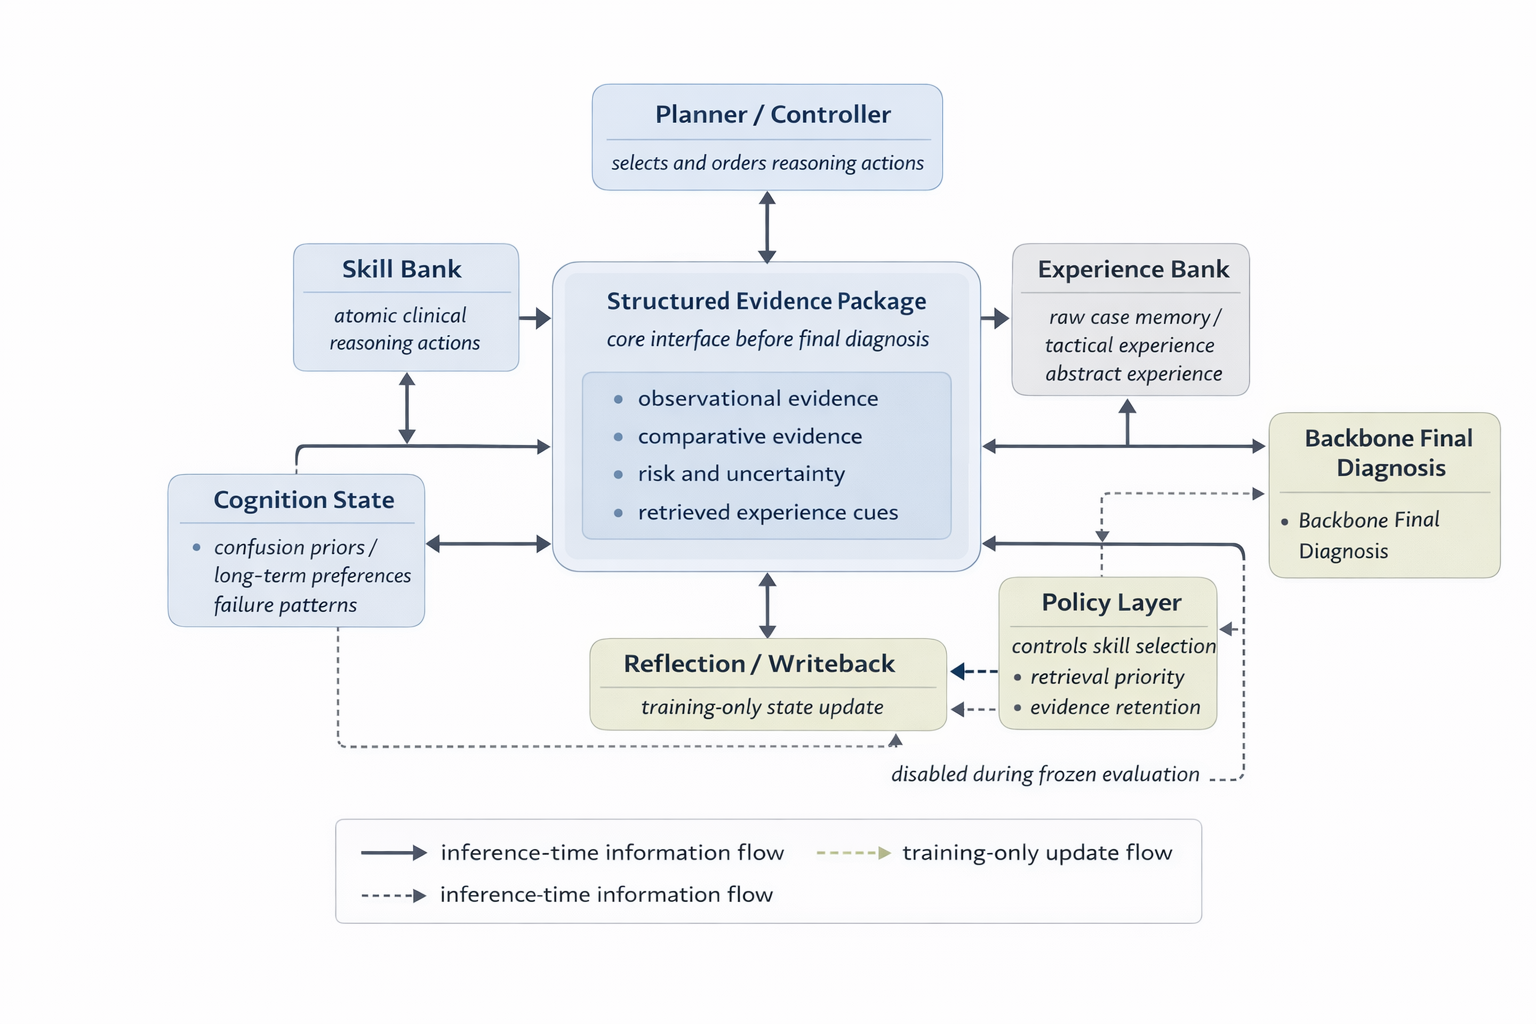
\includegraphics[width=0.9\textwidth]{figures/image6.png}}
    {\figureplaceholder{图2文件缺失：figures/image6.png}{0.24\textheight}}
  \caption{DermAgent 的内部状态结构与证据交互机制。该图强调技能库、经验库、认知状态与策略层如何共同影响当前病例的证据选择与组织，以及病例结果如何在训练阶段通过反思/写回回流到经验与认知层。}
  \label{fig:internal}
\end{figure*}

病例运行结束后，reflection/writeback 会将新的 outcome、skill helpfulness 与经验候选写回到 experience 与 cognition 中；在训练或版本化阶段，policy 层可以基于这些执行记录进行保守更新。在正式 frozen evaluation 中，在线 writeback 被关闭、split state 被固定，从而避免评测样本通过状态污染影响后续病例。

这里需要特别说明 writeback 的使用边界。DermAgent 并非在所有运行场景中都强制关闭状态写回；相反，在经验累积、候选策略开发或非正式运行阶段，writeback 可以开启，用于扩充经验库并更新认知状态。扩充的对象并不是单一的“历史样本缓存”，而是包括原始病例记忆、局部条件到动作的战术经验，以及跨病例抽象出的高层模式。只有在正式的 frozen evaluation 中，系统才显式关闭在线写回，并对 split state 进行固定快照。也就是说，DermAgent 既保留了经验增长与自演化的结构能力，也通过冻结协议确保正式比较不受在线状态污染影响；其“自演化”主要体现在积累阶段与训练阶段，而不是在正式测试样本上边评测边更新。换句话说，累计阶段可以打开 writeback，而正式运行中的冻结评测阶段必须关闭 writeback；本文需要比较的是固定状态下的 agent 增益，而不是在线适应该批测试样本后的增益。

\subsection{训练与优化}

DermAgent 的训练目标并不是对骨干视觉语言模型进行 finetuning，也不是端到端重训练诊断模型。本文将优化重点放在 frozen-backbone 条件下的外围 policy layer，即那些决定“哪些 skills 被调用”“哪些经验被优先使用”“哪些 structured evidence 被保留并进入最终诊断上下文”的中间策略组件。主要可训练对象包括 controller、retrieval reranker/scorer 与 evidence calibrator。训练信号来自 execution records、frozen split state、helpful/harmful signals 以及 downstream evaluation-oriented supervision。为保证可归因性，训练采用 staged pipeline，而不是将所有外围模块放入统一黑箱中联合优化。

这里也需要强调一个边界：本文当前结果已经证明经验状态可以被保存、回放与再次用于后续病例，但并未把“经验复用带来的长期累计收益曲线”作为独立实验主结果报告。因此，本文对经验可复用性的主张首先建立在系统设计、状态管理与冻结/非冻结运行机制之上，而关于经验资产在更长时间尺度上的收益累积，仍属于后续应继续量化验证的方向。

\subsection{冻结评测设置}

为了评估结构化 agent reasoning 相对于 direct prompting 的真实增益，本文采用 frozen evaluation。正式评测时，在线 writeback 被关闭，系统不允许在评测过程中将当前病例的反思结果继续写回 experience bank 或 cognition state；同时，split state 被固定。除此之外，baseline 与 agent 共享相同的 backbone、相同的 case list、相同的输入可见条件与一致的病例顺序，从而尽可能消除不公平比较与状态污染对结论的干扰。

\section{实验设置}

\subsection{数据集与标签空间}

实验围绕皮肤科图像诊断任务构建，输入由病灶图像及可选临床 metadata 组成。本文主实验使用 \texttt{pad\_ufes\_20} 数据，并采用固定划分 \texttt{pad\_ufes\_20\_contiguous\_v1}。数据按 70\%/15\%/15\% 划分为 train/val/test，并以确定性 case list 支持 frozen evaluation 与重复运行的一致性。

本文使用六类标准化 dermatology label space：\texttt{BCC}、\texttt{ACK}、\texttt{NEV}、\texttt{SEK}、\texttt{SCC} 和 \texttt{MEL}。恶性相关评测中，\texttt{BCC}、\texttt{ACK}、\texttt{SCC} 和 \texttt{MEL} 被视为 malignant 或 clinically high-risk labels，而 \texttt{NEV} 与 \texttt{SEK} 被视为 benign labels。

\subsection{骨干模型、基线与评测协议}

本文的主 baseline 为 direct Qwen baseline，即在与 DermAgent 完全相同的 backbone/service、输入条件和病例列表下，不启用经验检索、skill selection、evidence package、reflection/writeback 等中间层，而直接由 Qwen 输出最终诊断。这一 baseline 与本文的研究问题严格对应，因为它回答的是：在底层模型保持不变时，引入结构化 agent reasoning 是否带来增益。

正式比较遵循 same-backbone comparison、matched-case comparison 与 frozen-state constraints。所有正式 agent-vs-baseline 比较都基于完全相同的 case list、相同的病例顺序、相同的数据 split 以及一致的输入可见条件。

\subsection{实现说明}

系统以冻结 backbone、可替换外围策略模块的方式实现。主实验采用相同的 Qwen 骨干服务，并在 matched-case、matched-protocol 条件下比较 direct baseline 与 agent variants；额外对照中，我们还将相同的 agent scaffold 迁移到 SkinVL 骨干上，以评估方法的跨骨干可迁移性。所有正式结果均在 frozen evaluation 协议下导出，即固定 case list、禁止在线 writeback，并保持相同输入可见条件与病例顺序。与之相对，在经验累积与策略开发阶段，系统允许启用 reflection/writeback，以便将单次病例中的有效技能使用、典型混淆与高价值证据模式沉淀为后续可复用的状态资产。换言之，本文实际区分了两个运行阶段：用于形成与扩充经验/认知资产的累积阶段，以及用于公平比较 agent-vs-baseline 的正式冻结评测阶段；只有后者要求运行期间严格关闭在线写回。

\section{实验结果}

\subsection{主受控对比：DermAgent 与直接 Qwen 基线}

本节报告完整 DermAgent 与直接 Qwen 基线在同骨干比较、相同 345 个测试病例以及冻结评测条件下的主结果。基础服务在两组之间保持一致，均使用同一 Qwen 服务与相同病例列表；智能体组额外启用结构化推理支架、分层经验库、动态技能选择与证据组织。

\begin{figure*}[t]
  \centering
  \IfFileExists{figures/figure3_main_results_bar.png}
    {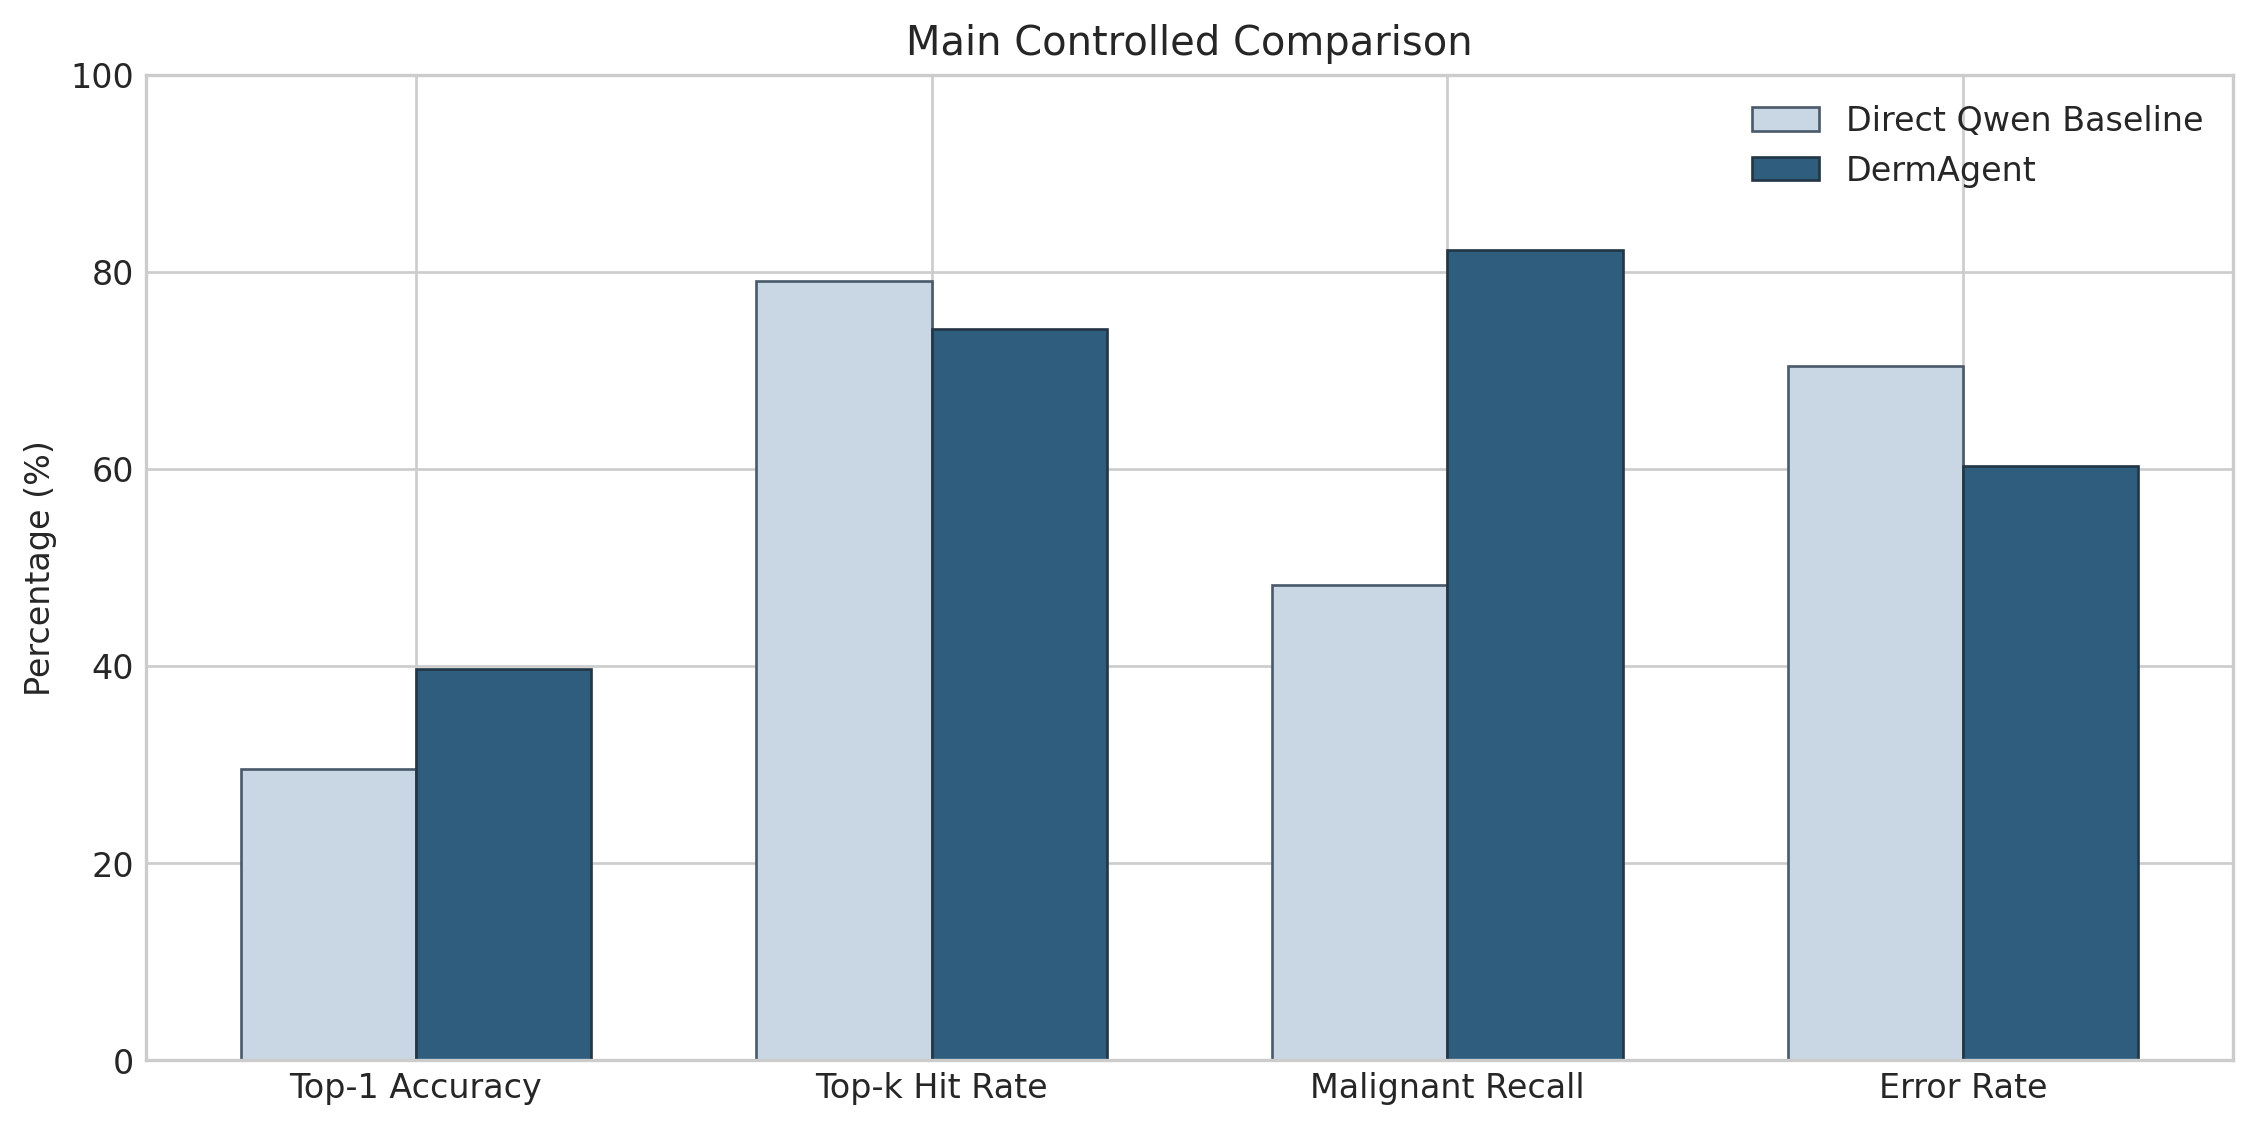
\includegraphics[width=0.82\textwidth]{figures/figure3_main_results_bar.png}}
    {\figureplaceholder{主结果概览图文件缺失：figures/figure3_main_results_bar.png}{0.20\textheight}}
  \caption{DermAgent 与直接 Qwen 基线的主结果对比。该图展示两种系统在 Top-1 Accuracy、Top-k Hit Rate、Malignant Recall 与 Error Rate 上的整体表现。}
  \label{fig:main_results_overview}
\end{figure*}

当前已完成的主对比结果如下：直接 Qwen 基线在 345 个带有真实标签的测试病例上达到 top-1 = 102/345 (29.6\%)、top-k = 273/345 (79.1\%)、恶性召回 = 133/276 (48.2\%)、错误率 = 243/345 (70.4\%)。在完全匹配的同骨干比较条件下，DermAgent 达到 top-1 = 137/345 (39.7\%)、top-k = 256/345 (74.2\%)、恶性召回 = 227/276 (82.2\%)、错误率 = 208/345 (60.3\%)。相对于基线的变化分别为：top-1 +10.1 个百分点、恶性召回 +34.1 个百分点、错误率 -10.1 个百分点，而 top-k 为 -4.9 个百分点。

\begin{table*}[t]
\centering
\caption{在相同骨干、相同 345 个测试病例与冻结评测条件下，DermAgent 与直接 Qwen 基线的主对比结果。}
\label{tab:main_results}
\small
\begin{tabular}{lccc}
\toprule
指标 & 直接 Qwen 基线 & DermAgent & 变化 \\
\midrule
Top-1 准确率 & 102/345 = 29.6\% & 137/345 = 39.7\% & +10.1 个百分点 \\
Top-k 命中率 & 273/345 = 79.1\% & 256/345 = 74.2\% & -4.9 个百分点 \\
恶性召回率 & 133/276 = 48.2\% & 227/276 = 82.2\% & +34.1 个百分点 \\
错误率 & 243/345 = 70.4\% & 208/345 = 60.3\% & -10.1 个百分点 \\
\bottomrule
\end{tabular}
\end{table*}

这些结果表明，在固定骨干的条件下，DermAgent 在 top-1 准确率、恶性召回率与错误率上都表现出明确改善，尤其是在恶性相关召回上获得了较大幅度提升。与此同时，top-k 的下降也说明当前智能体推理支架可能在提高最终决断集中度的同时牺牲了部分鉴别候选覆盖范围，因此不能将本轮结果简单概括为“所有指标均改善”。更准确地说，当前结果主要支持 DermAgent 在最终判断质量与高风险纠错上的增益，而不支持其在所有候选覆盖指标上无条件占优；也正因为如此，本文后续的 claim 需要明确限定在 top-1 纠错、高风险病例识别与可审计证据组织上，而不是泛化为“整套系统在所有指标上都稳定最优”。

\subsection{病例级配对统计}

为了避免总体比例掩盖逐病例层面的变化，我们进一步对 345 个测试病例进行了配对统计分析。结果显示，DermAgent 在 top-1 准确率上有 86 个病例实现了“基线错、智能体对”的纠正，而基线仅在 51 个病例上占优；在恶性召回率上，仅智能体正确为 103 例，而仅基线正确仅为 8 例。相比之下，top-k 命中率上则是仅基线正确 42 例、仅智能体正确 26 例，说明 top-k 的下降主要来自部分病例上的候选覆盖收缩。

\begin{table*}[t]
\centering
\caption{345 个配对病例上的配对统计（McNemar 精确检验）。其中“仅智能体正确”表示仅 DermAgent 正确，“仅基线正确”表示仅直接 Qwen 基线正确。}
\label{tab:paired_stats}
\small
\begin{tabular}{lccccc}
\toprule
指标 & 二者都正确 & 仅基线正确 & 仅智能体正确 & 二者都错误 & $p$ 值 \\
\midrule
Top-1 准确率 & 51 & 51 & 86 & 157 & 0.0035 \\
Top-k 命中率 & 230 & 42 & 26 & 47 & 0.0681 \\
恶性召回率 & 124 & 8 & 103 & 110 & $3.68\times10^{-22}$ \\
错误率 & 157 & 86 & 51 & 51 & 0.0035 \\
\bottomrule
\end{tabular}
\end{table*}

McNemar 精确检验进一步表明，top-1 准确率与错误率的改善具有统计显著性，而恶性召回率的提升则极为显著。这说明 DermAgent 的主要优势不是简单扩大候选集合，而是在逐病例层面更稳定地纠正最终 top-1 预测，并显著减少恶性相关漏检。

\subsection{图像读取作用审计}

鉴于 DermAgent 在系统设计上显式区分了“骨干模型负责看图与最终诊断”和“agent 负责结构化证据增强”，我们进一步进行了一个小规模图像读取审计实验，用于验证最终结果是否真的受到图像输入影响，而不仅仅是受到 metadata 或中间证据模板的驱动。具体做法是：在 \texttt{pad\_ufes\_20} 的 50 个测试病例上，对同一病例分别运行标准的有图版本与去除图像输入的 text-only counterfactual 版本，并保持其余 agent 流程、策略配置与冻结状态不变；随后统计两种运行在最终结果层面的差异。这里我们区分两类指标：其一是 \emph{result changed}，即去除图像后最终诊断标签是否发生变化；其二是 \emph{quality changed}，即去除图像后是否进一步改变了 top-1 正误或恶性召回成败。

结果显示，在 50 个病例中，有图与无图条件下共有 30 例（60.0\%）出现最终结果变化，11 例（22.0\%）进一步表现为结果质量变化；若只看 agent 运行中的内置 counterfactual 审计，对应数字分别为 35 例（70.0\%）与 13 例（26.0\%）。两组统计量数量级接近，说明该审计并非仅由局部 prompt 扰动驱动，而是能够在整条 agent 推理链上稳定地反映图像输入的作用。更重要的是，质量变化并非单向有利：部分病例中图像帮助系统把 \texttt{SEK}/\texttt{NEV} 等误判修正为正确标签，也有少数病例中图像线索会把结果从 text-only 条件下的正确答案带偏。这一现象表明，DermAgent 的最终输出并不是在“无图也几乎一样”的伪多模态模式下工作，而是确实在相当一部分病例上利用了视觉输入；同时，它也提示图像证据对最终决策既可能提供增益，也可能在少数边界病例上引入新的偏置。

\subsection{定性案例分析}

定性案例与上述统计结果相一致。以 \texttt{PAT\_73\_111} 为例，其 ground truth 为 \texttt{BCC}，direct Qwen 将其判断为 \emph{Seborrheic Keratosis}，而 DermAgent 在 morphology、border/surface、temporal evolution 与 malignancy risk assessment 等 skills 支持下，将最终诊断修正为 \emph{Basal Cell Carcinoma}，同时把恶性召回由失败修正为成功。另一例 \texttt{PAT\_1492\_1705} 的 ground truth 为 \texttt{ACK}，baseline 将其误判为 \emph{Contact Dermatitis} 且 top-k 未覆盖正确标签；agent 则在 metadata consistency、malignancy risk assessment 与经验检索支持下，将结果修正为 \emph{Actinic Keratosis}，实现了 top-1、top-k 与 malignant recall 的同步改善。

与此同时，失败案例也揭示了当前系统的偏差来源。在 \texttt{PAT\_100\_393} 中，真实标签为 \texttt{NEV}，基线正确输出 \emph{Nevus}，而智能体在风险信号与高不确定性上下文影响下将其上调为 \emph{Malignant Melanoma}。这说明结构化证据虽然有助于纠正高风险漏检，但在部分边界性良性病例上也可能引入过度警觉。因此，DermAgent 的定性证据更准确的解读应是：其主要收益来自高风险纠错与证据重组，而主要风险则是对少数良性病例的风险上调。

\subsection{技能与经验的阶段性贡献}

为了进一步分析系统收益来自何处，我们在与主实验相同的 345 个测试病例上进行了阶段性构建实验，依次比较直接 Qwen 基线、仅保留基础技能的第一阶段版本、引入技能库但不启用经验层的版本，以及引入经验但不启用高级专科技能的版本。表~\ref{tab:stagewise_results} 给出了结果。

\begin{figure}[t]
  \centering
  \IfFileExists{figures/figure4_stagewise_contributions.png}
    {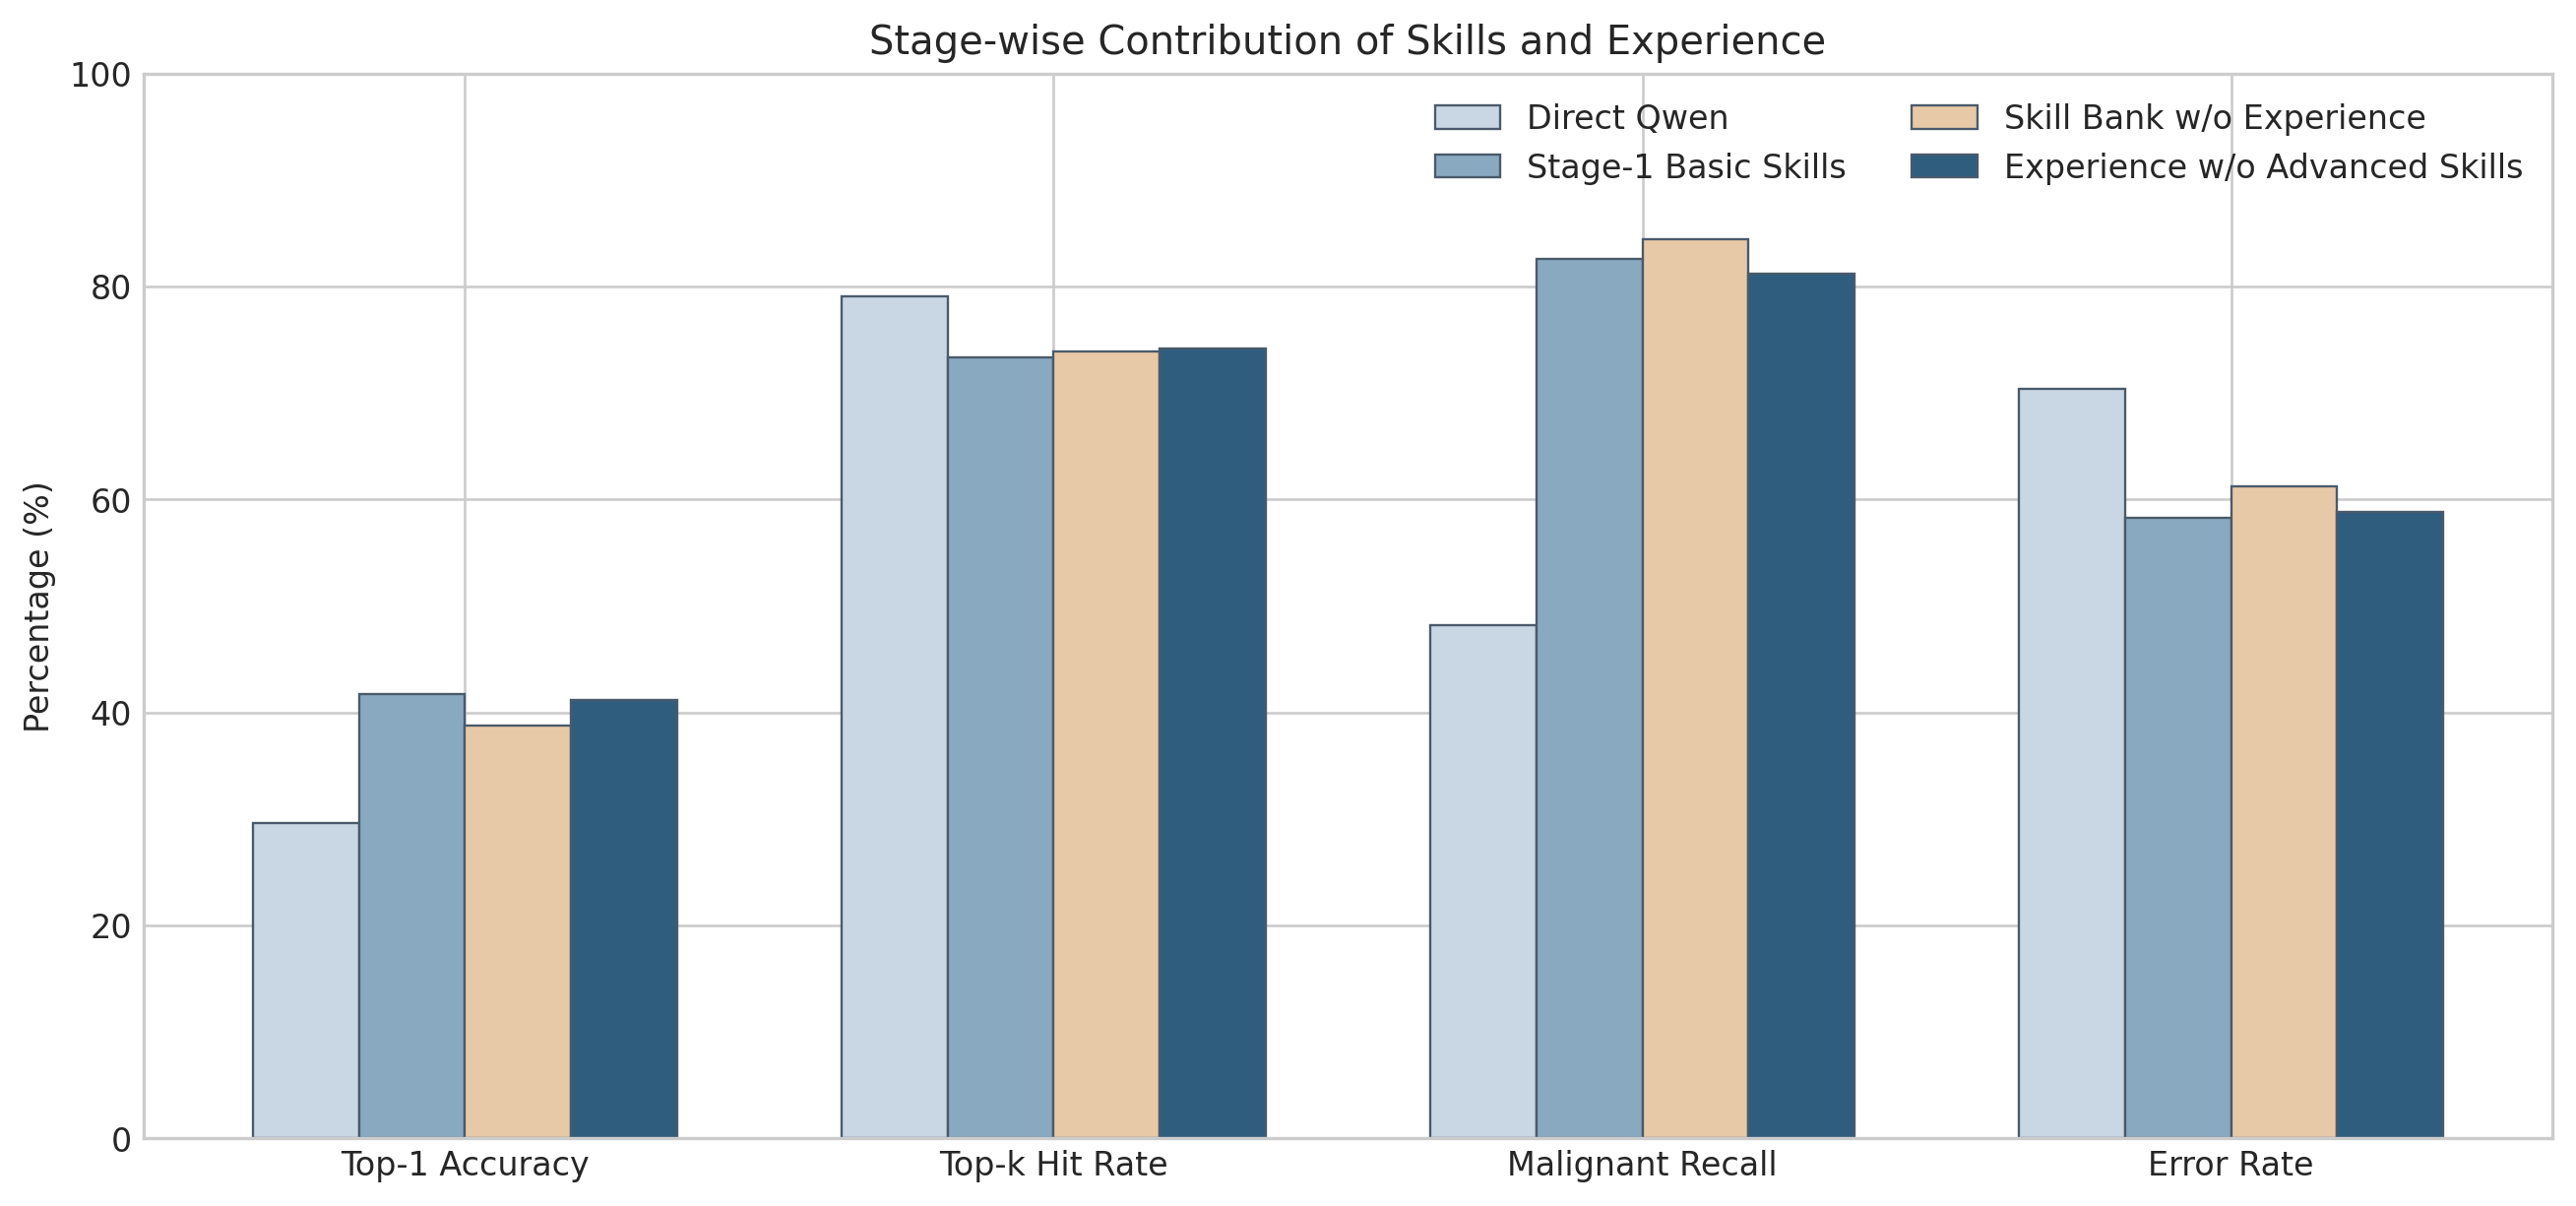
\includegraphics[width=\columnwidth]{figures/figure4_stagewise_contributions.png}}
    {\figureplaceholder{阶段性贡献图文件缺失：figures/figure4_stagewise_contributions.png}{0.20\textheight}}
  \caption{技能与经验的阶段性贡献。该图比较了直接 Qwen、第一阶段基础技能、无经验的技能库以及无高级技能的经验版本在主要指标上的差异。}
  \label{fig:stagewise_contributions}
\end{figure}

\begin{table}[t]
\centering
\caption{在 345 个测试病例上的阶段性构建实验。}
\label{tab:stagewise_results}
\begin{adjustbox}{max width=\columnwidth}
\scriptsize
\begin{tabular}{lcccc}
\toprule
指标 & 直接 Qwen & 第一阶段基础技能 & 无经验的技能库 & 无高级技能的经验版 \\
\midrule
Top-1 准确率 & 29.6\% & 41.7\% & 38.8\% & 41.2\% \\
Top-k 命中率 & 79.1\% & 73.3\% & 73.9\% & 74.2\% \\
恶性召回率 & 48.2\% & 82.6\% & 84.4\% & 81.2\% \\
错误率 & 70.4\% & 58.3\% & 61.2\% & 58.8\% \\
\bottomrule
\end{tabular}
\end{adjustbox}
\end{table}

这一结果呈现出三个值得注意的现象。第一，仅引入基础技能库即可将 top-1 准确率从 29.6\% 提升到 41.7\%，同时将恶性召回率从 48.2\% 提升到 82.6\%，说明本文在前文方法部分强调的核心设计确实成立：将观察、比较、风险评估与不确定性审计这些基础临床动作显式化，本身就能为最终诊断提供高价值结构化证据。第二，仅有技能库而无经验的版本在恶性召回率上达到 84.4\%，是这一组实验中的最高值，提示经验检索并不是唯一收益来源，技能触发和证据路由的质量同样关键。第三，在加入经验但移除高级专科技能后，系统仍保持 41.2\% 的 top-1 准确率和 81.2\% 的恶性召回率，说明分层经验与基础临床推理技能已能贡献大部分收益，而专科技能主要进一步改善特定高混淆场景。

这一阶段性结果也提示，本文不宜把贡献简单表述为“skills、experience、cognition 与 controller 的每一层都会在所有指标上带来单调增益”。更合理的解释是：基础 clinical reasoning skills 构成了主要性能来源，而经验、认知与控制器更多是在稳定性、风险识别、效率压缩与特定混淆场景中提供附加价值。换言之，这组实验确实揭示了框架中存在“基础层已贡献主体收益、后续层提供条件性附加收益”的结构，因此不能把完整框架的有效性 claim 写得过满。

\subsection{完整系统组件消融}

在完成完整 DermAgent 的基础上，我们又在一个 100 例的冻结对照子集上进行了更细粒度的组件消融，用于分析认知更新、抽象经验、专科技能以及不同控制器设计的作用。结果如表~\ref{tab:ablation_full} 所示。

\begin{figure}[t]
  \centering
  \IfFileExists{figures/figure5_subset100_ablation.png}
    {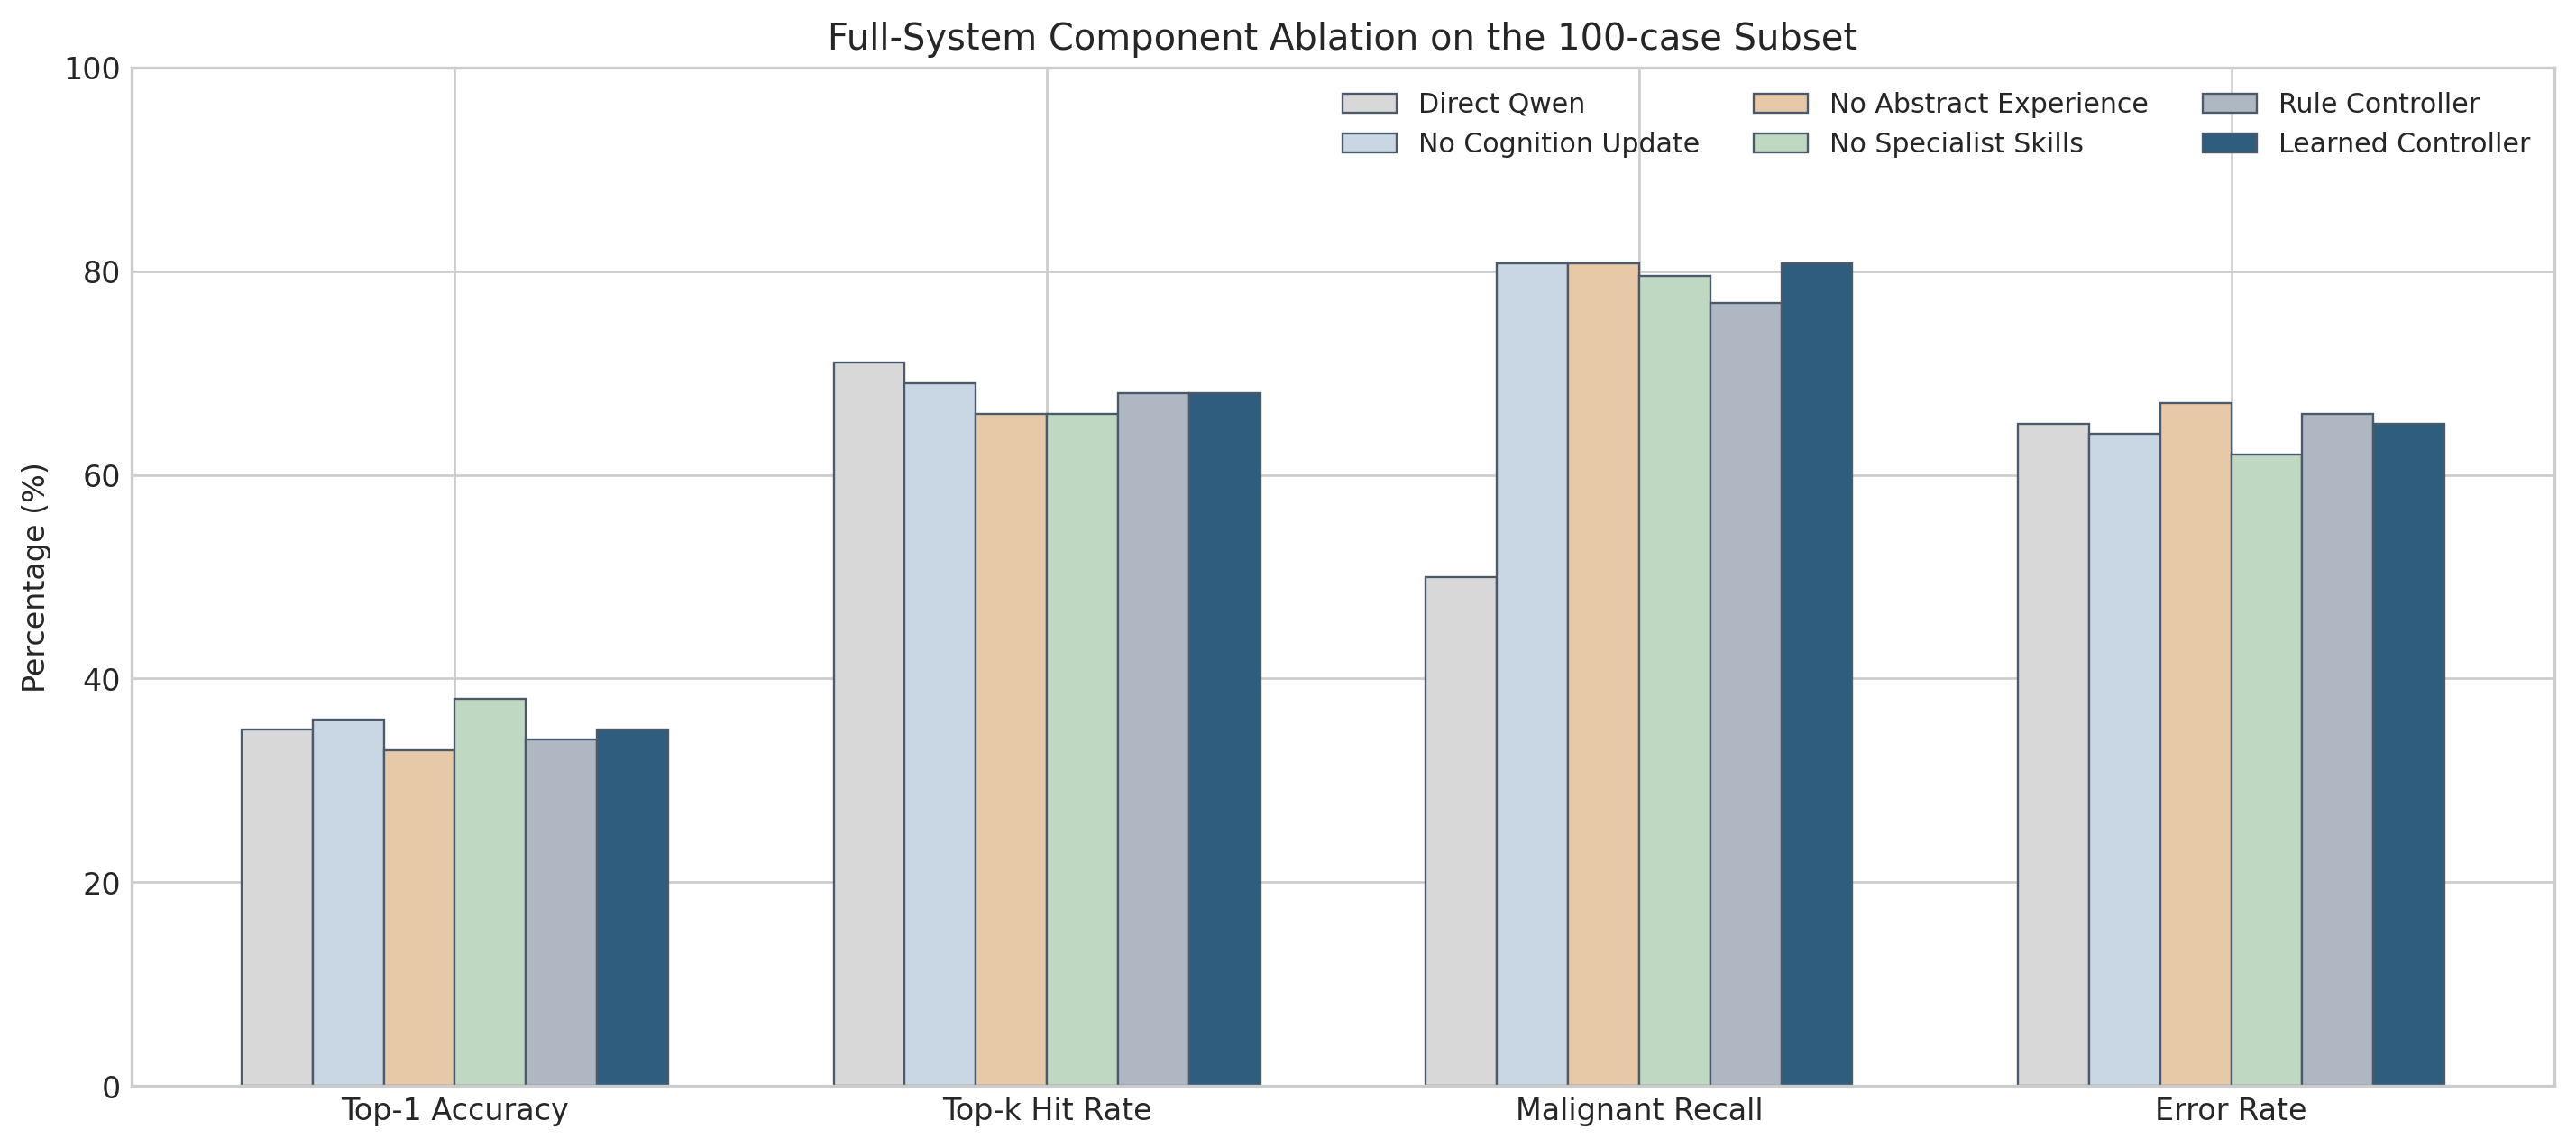
\includegraphics[width=\columnwidth]{figures/figure5_subset100_ablation.png}}
    {\figureplaceholder{100例消融图文件缺失：figures/figure5_subset100_ablation.png}{0.20\textheight}}
  \caption{100 例子集上的完整系统组件消融。该图展示不同组件去除或控制器替换后，系统在主要指标上的变化。}
  \label{fig:subset100_ablation}
\end{figure}

\begin{table}[t]
\centering
\caption{100 个病例子集上的完整系统组件消融。}
\label{tab:ablation_full}
\begin{adjustbox}{max width=\columnwidth}
\scriptsize
\begin{tabular}{lcccccc}
\toprule
指标 & 直接 Qwen & 无认知更新 & 无抽象经验 & 无专科技能 & 规则控制器 & 学习控制器 \\
\midrule
Top-1 准确率 & 35.0\% & 36.0\% & 33.0\% & 38.0\% & 34.0\% & 35.0\% \\
Top-k 命中率 & 71.0\% & 69.0\% & 66.0\% & 66.0\% & 68.0\% & 68.0\% \\
恶性召回率 & 50.0\% & 80.8\% & 80.8\% & 79.5\% & 76.9\% & 80.8\% \\
错误率 & 65.0\% & 64.0\% & 67.0\% & 62.0\% & 66.0\% & 65.0\% \\
\bottomrule
\end{tabular}
\end{adjustbox}
\end{table}

从该表可以看出，去除抽象经验会使 top-1 准确率降至 33.0\%，同时错误率升至 67.0\%，说明跨病例抽象经验对于稳定最终判断仍然重要。去除认知更新后，top-1 仅为 36.0\%，也提示认知状态并非冗余缓存，而是会实质影响技能使用与证据路由。去除专科技能时，top-1 准确率为 38.0\%，在该子集上仍保持较强表现，说明专科技能的作用更偏向细粒度风险甄别与混淆纠错，而不是唯一决定整体性能的核心来源。

控制器的指标增益整体较为有限，但学习控制器在当前子集上表现出轻微的正向趋势：其恶性召回率为 80.8\%，略高于规则控制器的 76.9\%，而 top-1 准确率与 top-k 命中率基本持平。这里还需要直接解释一个表面上容易令人困惑的现象：在该 100 例子集上，去除专科技能时 top-1 准确率为 38.0\%，而学习控制器版本为 35.0\%。这一差异并不意味着“去掉控制器一定更好”，而是说明控制器优化的目标并不是在每个局部子集上追求最高的单点 top-1，而是更精准地选择少量关键 skills。也正因为如此，在当前最新版控制器设置下，系统每例实际触发的技能数量可由约 11--13 个压缩到 3--5 个，减少将近 10 个 skills，在主要指标基本保持稳定的前提下显著降低了推理开销。相较于这种明显的速度与成本收益，子集上有限的 top-1 波动更适合被理解为整体系统优化中的可接受代价，而不是对控制器价值的否定。换言之，控制器在本文中的主要角色首先是“更精准地选取少量高价值 skills，以压缩中间推理开销”，其次才是在某些设定下争取额外的准确率收益；因此，它在方法部分就应被理解为效率控制层，而不是主要依赖最终准确率证明自身价值的核心分类增益模块。

\subsection{向专用皮肤病骨干模型迁移}

除 Qwen 主骨干外，我们还将同一智能体推理支架迁移到专用皮肤病大模型 SkinVL 上进行验证，以考察 DermAgent 是否能在专用皮肤病骨干模型上继续带来增益。表~\ref{tab:skinvl_results} 给出了 333 个病例上的对照结果。

\begin{figure}[t]
  \centering
  \IfFileExists{figures/figure6_skinvl_transfer.png}
    {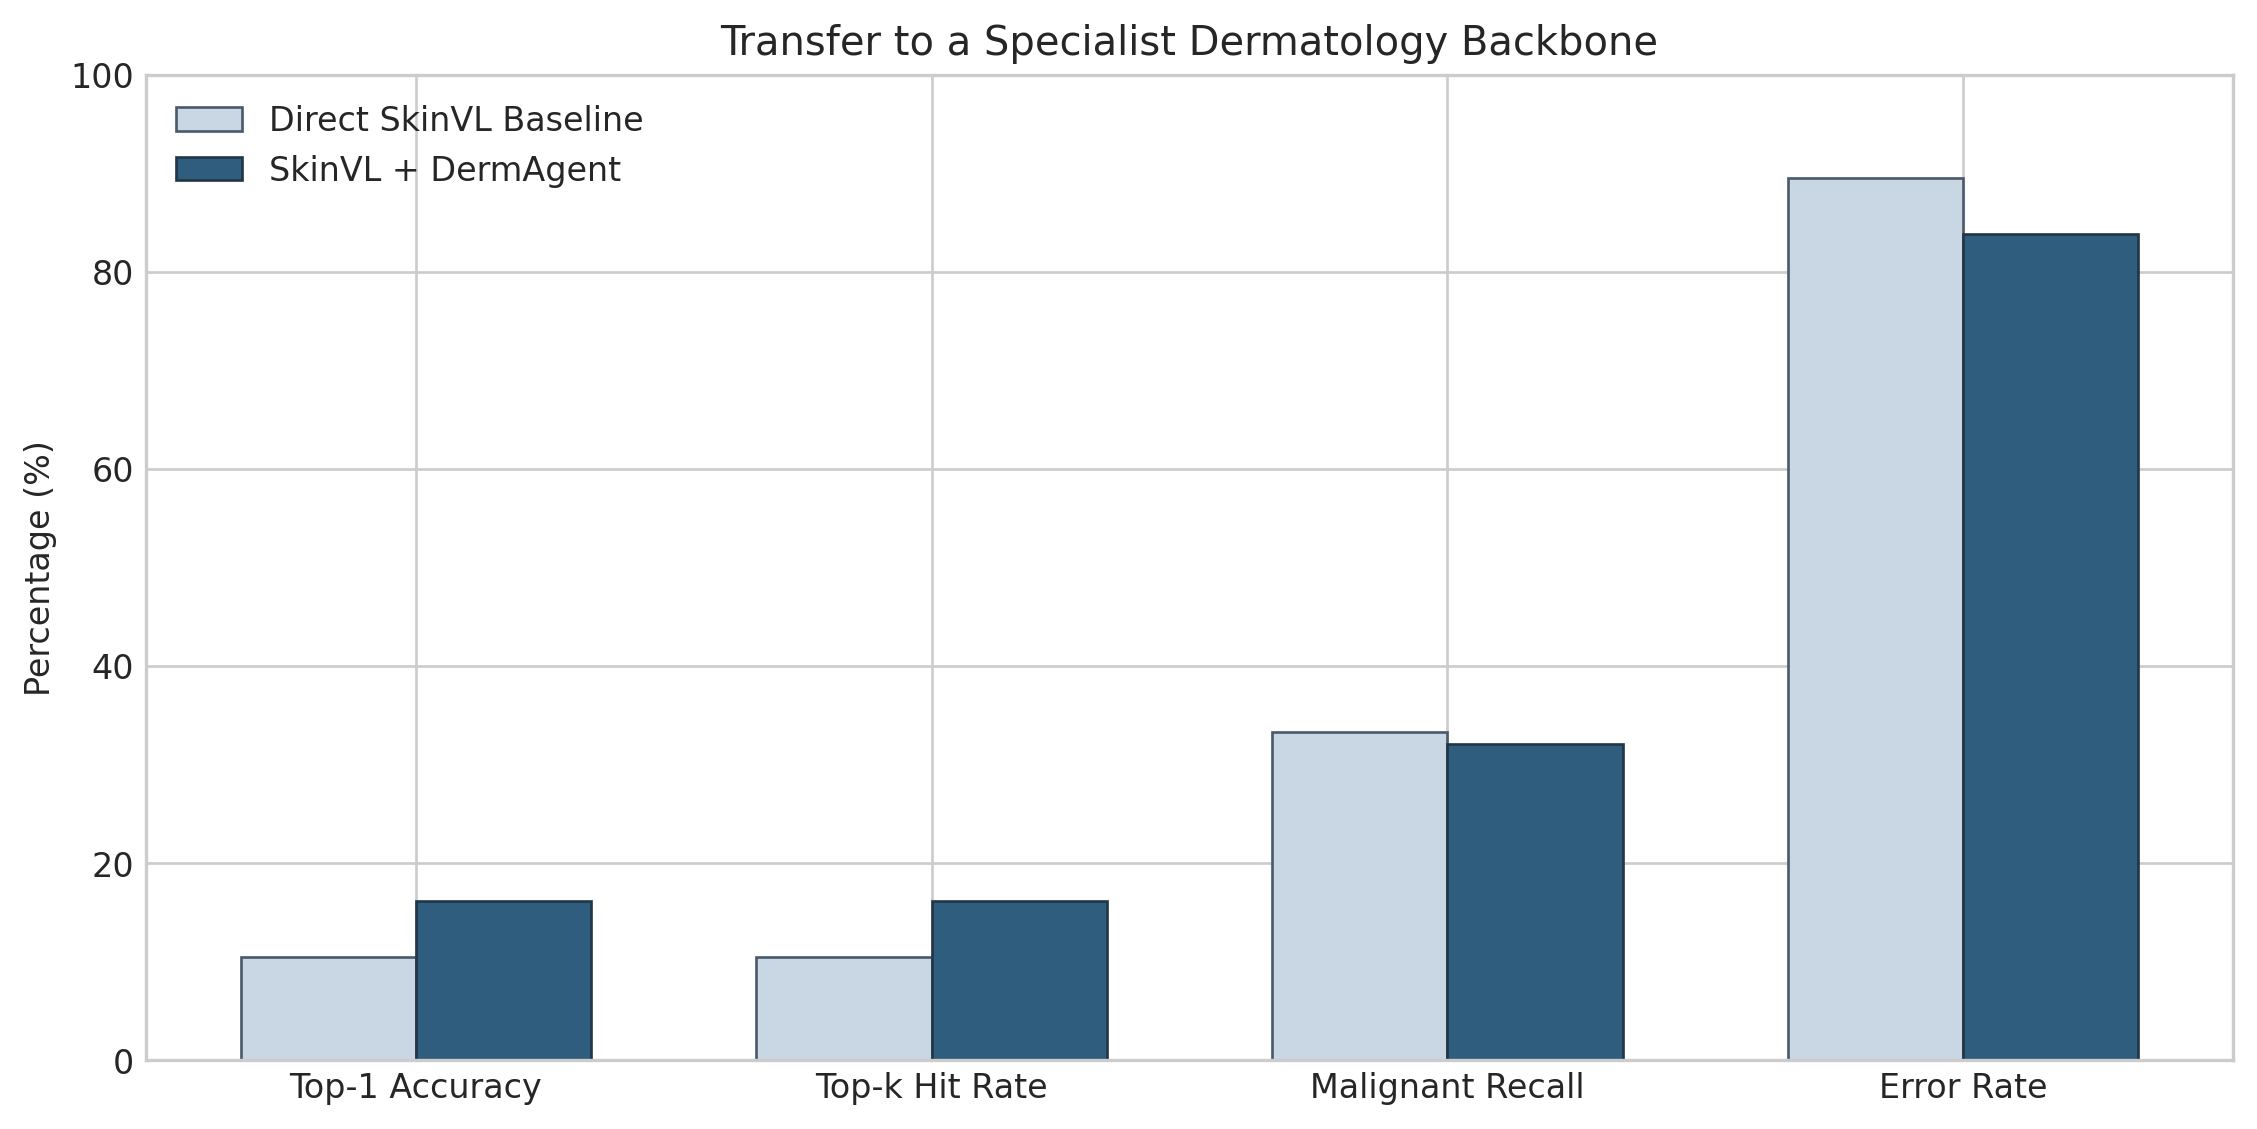
\includegraphics[width=\columnwidth]{figures/figure6_skinvl_transfer.png}}
    {\figureplaceholder{SkinVL迁移图文件缺失：figures/figure6_skinvl_transfer.png}{0.20\textheight}}
  \caption{DermAgent 向专用皮肤病骨干模型 SkinVL 的迁移结果。该图展示直接 SkinVL 基线与 SkinVL + DermAgent 在主要指标上的对比。}
  \label{fig:skinvl_transfer}
\end{figure}

\begin{table}[t]
\centering
\caption{SkinVL 专用皮肤病骨干上的智能体推理支架对照结果。}
\label{tab:skinvl_results}
\begin{adjustbox}{max width=\columnwidth}
\footnotesize
\begin{tabular}{lccc}
\toprule
指标 & 直接 SkinVL 基线 & SkinVL + DermAgent & 变化 \\
\midrule
Top-1 准确率 & 35/333 = 10.5\% & 54/333 = 16.2\% & +5.7 个百分点 \\
Top-k 命中率 & 35/333 = 10.5\% & 54/333 = 16.2\% & +5.7 个百分点 \\
恶性召回率 & 111/333 = 33.3\% & 107/333 = 32.1\% & -1.2 个百分点 \\
错误率 & 298/333 = 89.5\% & 279/333 = 83.8\% & -5.7 个百分点 \\
\bottomrule
\end{tabular}
\end{adjustbox}
\end{table}

结果表明，DermAgent 在 SkinVL 这一专用皮肤病大模型上同样能够带来明显增益：top-1 准确率从 10.5\% 提升到 16.2\%，top-k 命中率也从 10.5\% 提升到 16.2\%，错误率从 89.5\% 降至 83.8\%。这说明本文提出的结构化证据推理支架并不只对通用 Qwen 骨干有效，在专用皮肤病骨干模型上也具有可观的增强作用。尽管该组实验中的恶性召回率从 33.3\% 略降至 32.1\%，但这一现象并不与主结论直接矛盾：它更说明外围策略的迁移收益具有骨干依赖性，尤其在高风险召回这一敏感指标上，仍需要根据不同 backbone 的生成特性进一步适配。一个更具体的可能解释是，当前外围策略的主要稳定版本是在 Qwen 主线上发展和筛选出来的，其风险相关 evidence weighting、skill triggering 与 evidence routing 逻辑更贴近 Qwen 的最终生成偏好；当同一支架直接迁移到 SkinVL 时，虽然 top-1 与错误率仍可受益，但恶性风险线索未必会以相同方式被最终诊断阶段吸收，因此会出现 recall 不完全同步改善的情况。换言之，这里的现象不是“agent 一定导致更多漏检”，而是“agent 在 SkinVL 上同时带来了部分恶性纠错与部分恶性漏失，其净结果表现为恶性召回未同步提升”，因此需要更细的 backbone-specific 风险策略适配。

\subsection{高覆盖候选条件下的调整实验}

我们还进行了一个较小规模的 60 例对照实验，用于检验在较强候选覆盖条件下进行假设性智能体调整是否会改变最终表现。结果如表~\ref{tab:hyp_adjust} 所示。

\begin{table}[t]
\centering
\caption{60 个病例上的假设性智能体调整对照。}
\label{tab:hyp_adjust}
\begin{adjustbox}{max width=\columnwidth}
\footnotesize
\begin{tabular}{lccc}
\toprule
指标 & 直接 Qwen 基线 & 假设性智能体调整 & 变化 \\
\midrule
Top-1 准确率 & 46/60 = 76.7\% & 45/60 = 75.0\% & -1.7 个百分点 \\
Top-k 命中率 & 58/60 = 96.7\% & 59/60 = 98.3\% & +1.7 个百分点 \\
错误率 & 14/60 = 23.3\% & 15/60 = 25.0\% & +1.7 个百分点 \\
\bottomrule
\end{tabular}
\end{adjustbox}
\end{table}

这一实验表明，当 baseline 本身已经具有很高的 top-1 与 top-k 覆盖时，额外的 agent adjustment 不一定继续改善最终 top-1，甚至可能因重排与收缩决策边界带来轻微退化。该结果与主实验并不矛盾，而是说明 agent 的收益具有条件依赖性：在困难病例、高风险病例和开放式 differential 较复杂的设置下，structured evidence 更容易发挥作用；而在候选空间已经较充分收敛的小规模对照中，其边际收益可能有限。

\section{Discussion}

DermAgent 的核心价值并不只是增加了一组中间模块，而在于为医学诊断场景中的智能体明确了角色边界。本文始终保持单一最终诊断者，即由骨干模型负责最终结论，而让智能体仅承担结构化证据增强与中间推理组织。这一设计首先带来清晰的责任边界。对于皮肤科诊断这类高风险、多混淆任务而言，如果外围模块同时拥有独立诊断权，再通过投票、加权或覆盖式决策决定最终输出，系统将很难回答“最终诊断究竟由谁负责”，也难以在错误分析中区分失败究竟来自骨干模型还是中间模块。

这一边界也解释了本文为什么坚持将 skill 设计为 reasoning action，而不是 disease classifier。若 skill 被设计为外围病种分类器，那么即便其局部性能较强，整个系统也会迅速滑向“多个模块共同猜病”的结构，导致中间层与 backbone 之间出现职责重叠。更重要的是，disease-specific 子分类器往往容易退化为刚性的 heuristic attachment。与之相比，将 skill 定义为 atomic clinical reasoning actions 可以更自然地对应真实诊断过程中的观察、比较、排除、风险评估与不确定性审计，使外围能力的优化对象从“病种输出”转变为“中间推理动作质量”。

本文的另一项核心设计，是将 experience bank、cognition state 与 policy layer 分层。这样做的意义并不只是软件架构上的整洁，而在于它为持续演化提供了更清晰的状态语义。experience 更偏向知识内容，回答的是系统从历史病例中保留了哪些具体案例、局部战术和抽象模式；cognition 更偏向策略状态，记录系统在跨病例尺度上形成了哪些偏好、混淆先验与行为统计；policy 则进一步把可训练、可版本化、可回滚的外围控制参数从经验内容和策略记忆中分离出来。

尽管如此，本文也应明确当前证据的边界。首先，DermAgent 在主实验中显著提升了 top-1 准确率与恶性召回率，但 top-k 命中率出现下降，说明系统当前更像是在“收缩并强化最终判断”，而非无条件扩大鉴别覆盖范围。其次，阶段性实验表明基础技能已能贡献大部分收益，这意味着经验、认知与控制器的价值应更谨慎地表述为稳定性、风险纠错、效率压缩与特定场景下的附加增益，而不是简单宣称整套模块在所有指标上都不可或缺。再次，控制器带来的准确率提升尚不显著，但其在当前最新版设置中的主要意义并不在于直接拉高最终分数，而在于将 skill 调用数由约 11--13 个显著压缩到 3--5 个，从而降低运行成本并提升系统可扩展性。最后，跨骨干实验虽然表明 DermAgent 在 SkinVL 上同样能够取得明显增益，但恶性召回率的变化并不完全一致，这提示外围策略仍需根据骨干特性进一步适配。

从更广义的方法学角度看，DermAgent 当前最有力的贡献并不是证明“更多模块一定带来更高分数”，而是证明在固定骨干条件下，存在一条不同于继续微调 backbone 的增强路线：通过资源更节制的外围策略优化，在保持最终诊断权边界清晰的同时，把 skill、experience 与状态更新沉淀为可复用资产。当前结果已经支持这一路线在主设定中的有效性，但对“经验复用带来的长期收益”与“不同骨干上的最优适配方式”，仍需要后续实验进一步展开。

值得指出的是，本文增加的图像读取审计也为系统边界提供了一个额外验证：在 50 个病例的对照中，去除图像后有 60.0\% 的病例最终结果发生变化，22.0\% 的病例进一步出现正确性或恶性召回变化。这说明 DermAgent 并不是主要依赖 metadata 或证据模板在“伪装成多模态推理”，而是在相当比例的病例上确实把图像输入带入了最终决策；但同样地，图像影响并不总是正向，这也提示未来仍需进一步改进视觉证据校准与高风险边界病例的稳健性。

总体而言，DermAgent 所提出的并非简单的提示工程变体，而是一种面向医学多模态诊断任务的结构化智能体设计范式：在保持骨干模型最终诊断权不变的前提下，将技能库、经验库、认知状态与策略层组织为可演化、可审计、可训练且可公平评测的外围推理支架。

\section{Conclusion}

本文提出 DermAgent，一个面向皮肤科多模态诊断的结构化智能体推理框架。与通过重新训练骨干模型或引入并行诊断器来提升性能的路线不同，DermAgent 保持皮肤科视觉语言模型骨干的最终诊断职责不变，而将技能、经验、认知与可训练外围策略层组织为最终诊断前的结构化证据推理支架。更准确地说，DermAgent 被定义为一个受边界约束的诊断智能体：它负责执行 test-time 结构化推理、组织中间证据并支持经验积累，但不夺取最终诊断权。本文的核心结论是：在固定骨干模型的前提下，将中间推理动作、分层经验、跨病例策略状态与证据组织过程显式化，能够以可审计、可分解且可公平比较的方式提升皮肤科诊断质量。

在受控实验中，DermAgent 在 345 个测试病例上将直接 Qwen 基线的 top-1 准确率从 29.6\% 提升到 39.7\%，将恶性召回率从 48.2\% 提升到 82.2\%，并将错误率从 70.4\% 降低到 60.3\%；配对统计进一步证明了 top-1 与恶性召回率增益的显著性。阶段性实验说明，基础临床推理技能已能贡献主要收益，而分层经验、抽象经验与认知更新则进一步提供稳定改进。组件消融与最新版控制器运行结果表明，控制器对最终指标的直接提升尚不显著，但其重要作用在于将每例 skill 调用数由约 11--13 个压缩到 3--5 个，从而显著提升推理效率。进一步地，DermAgent 在 SkinVL 这一专用皮肤病大模型上同样获得了 top-1 准确率与错误率的改善，说明本文提出的结构化推理支架具有跨骨干应用价值。与此同时，本文也明确保留结果边界：DermAgent 的主要收益体现在最终 top-1 判断质量、高风险纠错与过程可审计性上，而不是对所有候选覆盖指标或所有骨干设定的无条件同步提升。总体而言，本文结果支持这样一个结论：围绕固定皮肤科视觉语言模型骨干构建结构化、经验驱动的推理外骨骼，是一条具有真实实证价值和方法学意义的医学智能体研究方向。

此外，50 例图像读取审计显示，去除图像后有 60.0\% 的病例最终结果发生变化，22.0\% 的病例进一步出现正确性或恶性召回变化，从而为“DermAgent 的最终决策确实使用了视觉输入”提供了直接的行为层证据。这一结果使本文关于可审计多模态推理的主张更加完整：DermAgent 不仅在冻结骨干条件下提升了诊断性能，也能够通过 counterfactual 审计验证图像在最终结果中的实际作用。

\bibliographystyle{plainnat}
\bibliography{references}

\end{document}
